\subsection{Tablica cech wizualnych -- VFA}
\label{vfa}

VFA -- z angielskiego Visual Feature Array -- można to tłumaczyć jako tablica cech wizualnych. Autorom prac \cite{Csapo2006,Resko,Resko2005} spodobała się idea zaproponowana przez wspominanych wcześniej noblistów i zaproponowali model struktury powiązanych kolumn orientacyjnych, którą nazwali właśnie VFA.\\

Rysunek \ref{fig:vfa} przedstawia zaproponowany model tablicy cech wizualnych, w których w prostokąt oznaczony jako Input Image przedstawia obraz wejściowy. Jest on filtrowany i trafia do drugiego prostokąta, który reprezentuje ,,proste komórki'' w korze wzrokowej. Na tym etapie następuje integracja konturów. Gdy kontury zostaną zintegrowane, trafiają do etapu składania wyodrębnionych krawędzi w większe struktury.\\

%\begin{figure}[ht]
%	\centering
%	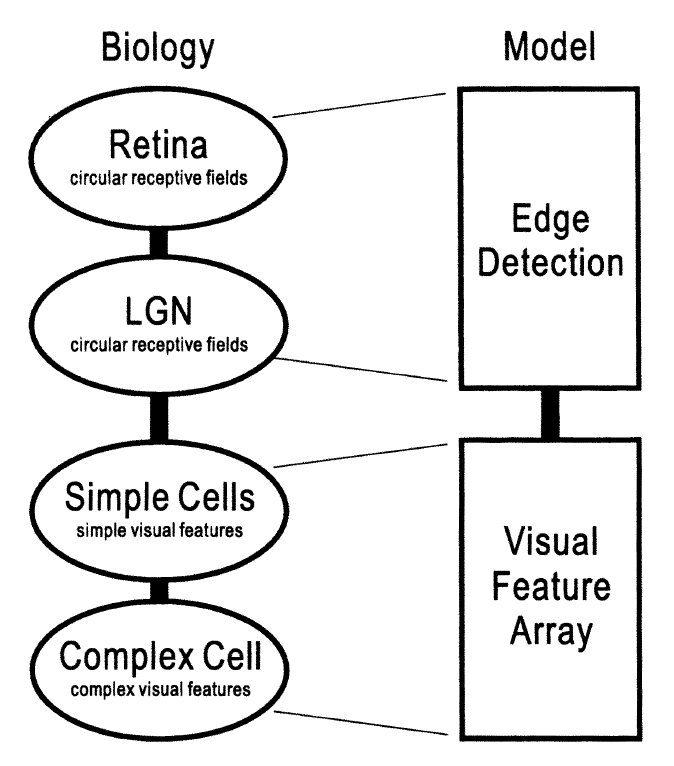
\includegraphics[width=.50\textwidth]{images/vfa_model_idea.png}
%	\caption{Przedstawienie szlaku wzrokowego wraz z pomysłem na model tablicy cech wizualnych \cite{Resko2005}.}
%	\label{fig:vfaIdea}
%\end{figure}

\begin{figure}[ht]
	\centering
	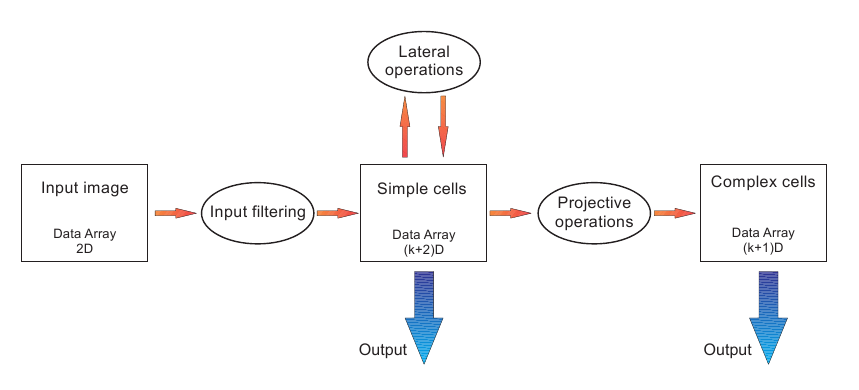
\includegraphics[width=1.00\textwidth]{images/vfa_model.png}
	\caption{Model tablicy cech wizualnych, prostokąty symbolizują struktury danych, elipsy natomiast transformacje \cite{Resko}.}
	\label{fig:vfa}
\end{figure}

\subsubsection{Filtrowanie\\}

Przy tym etapie -- wyodrębniania konturów -- autorzy stosują dosyć dobrze rozpowszechniony w grafice komputerowej filtr Gabora (załącznik \ref{aGabor}). Okazuje się, że natura w korze wzrokowej realizuje coś podobnego do tego matematycznego modelu, co jest opisane dosyć dobrze w pracy \cite{Jones1987}. Świadczy to o tym, że zastosowanie filtru Gabora jest bardzo dobrym krokiem ku celu, którym jest wykorzystanie zalet kory wzrokowej w rozpoznawaniu obrazów.

\subsubsection{Integracja konturów\\}

Na rysunku \ref{fig:vfa} opisana jako ,,Lateral operations''\footnote{Lateral Geniculate Nucleus -- z języka angielskiego -- ciało kolankowate boczne. Jest jednym z elementów szlaku wzrokowego -- którym informacja wizualna jest przenoszona do -- między innymi -- pierwotnej kory wzrokowej, chociaż połączeń jest dużo więcej niż tylko to z pierwszorzędową korą wzrokową. W sensie modelu określenie to ma symbolizować połączenia neuronów sąsiadujących będących w pewnym otoczeniu ze sobą.} integracja konturów, polega na tym, że neurony odpowiedzialne za krawędzie występujące w obrazie pod odpowiednim kątem mają fizyczne połączenie z neuronami odpowiedzialnymi za sąsiednie krawędzie, przez co wpływają na siebie nawzajem.\\

Autorzy założyli, że każda krawędź występująca w obrazie, a otrzymana w momencie ekstrakcji konturów miała przypisaną pewną wartość, która prezentuje jej istotność w obrazie. Wartość ta jest modyfikowana na skutek współdziałania neuronu odpowiedzialnego za tą krawędź z innymi, które z nim sąsiadują. Autorzy uznali, że dobrym podejściem będzie tutaj kombinacja liniowa istotności sąsiednich krawędzi w obrazie.

\subsubsection{Łączenie krawędzi i przedstawienie rezultatów\\}

Mimo, że autorzy dosyć dobrze przedstawili samą teorię potrzebną do realizacji poprzednich etapów, to budowanie cech złożonych -- które jest efektem łączenia krawędzi w większe struktury -- jak i szczegóły dotyczące wcześniejszych etapów jest traktowana po macoszemu -- o czym świadczy brak takich informacji w cytowanych pracach. Można odnieść wrażenie, że przedstawione są tutaj jedynie pomysły, a realizacja jest pozostawiona na uboczu.\\

Otrzymywane wyniki również specjalnie nie zachwycają, ponieważ nietrywialny przykład zastosowania jest tylko jeden, zaczerpnięty z pracy \cite{Resko2005}. 

\begin{figure}[ht]
	\centering
	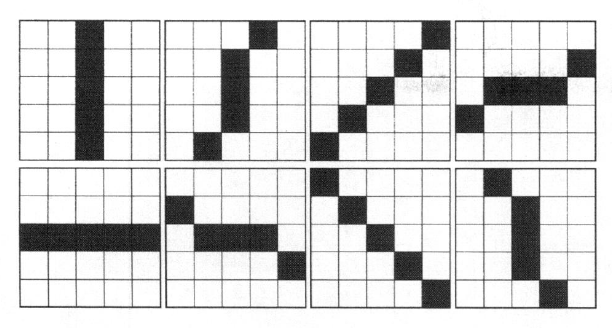
\includegraphics[width=.60\textwidth]{images/vfa_model_neurons.png}
	\caption{Krawędzie z modelu tablicy cech wizualnych, mające reprezentować krawędzie wyodrębnione w obrazie \cite{Resko2005}.}
	\label{fig:vfaModelNeurons}
\end{figure}

\begin{figure}[ht]
	\centering
	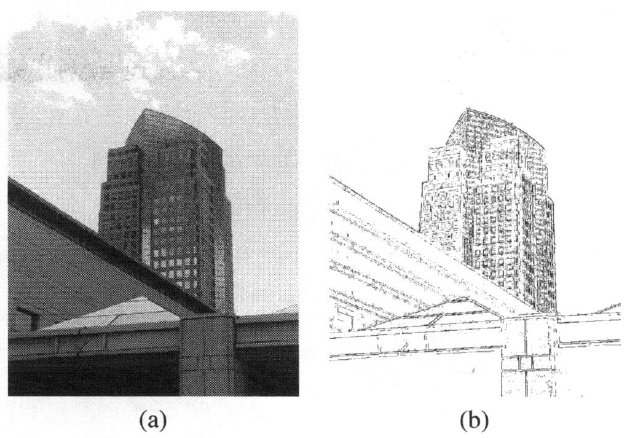
\includegraphics[width=.70\textwidth]{images/vfa_model_results.png}
	\caption{Rezultaty pracy modelu z obrazem: a) obraz wejściowy, b) wyjście z modelu \cite{Resko2005}.}
	\label{fig:vfaModelResults}
\end{figure}
